\documentclass[a4paper,10pt]{article}
\usepackage{hyperref}
\usepackage{float}
\usepackage{graphicx}

%%% Title
\title{Processo e Sviluppo Software: Assignment 3} 
\author{Ivo Junior Bettini - 806878, Umberto Cocca - 807191, \\Silvia Traversa - 816435\\
\href{https://gitlab.com/s.traversa/2019_assignment3_booksloan}{GitLab repository}}
\date{}

\begin{document}

\maketitle 


\section*{Applicazione BooksLoan}
L'applicazione proposta permette agli utenti di visualizzare il catalogo di una biblioteca. Essi possono visualizzare sia le copie disponibili, ed eventualmente richiederne una in prestito, sia quelle non disponibili e prenotarle per quando ritorneranno presso la biblioteca.
E' inoltre possibili visualizzare le informazioni relative ad ogni singolo libro, quali l'autore o la presenza di sequel. 

\section*{Schema E-R}

\begin{figure}[H]
	\centering
	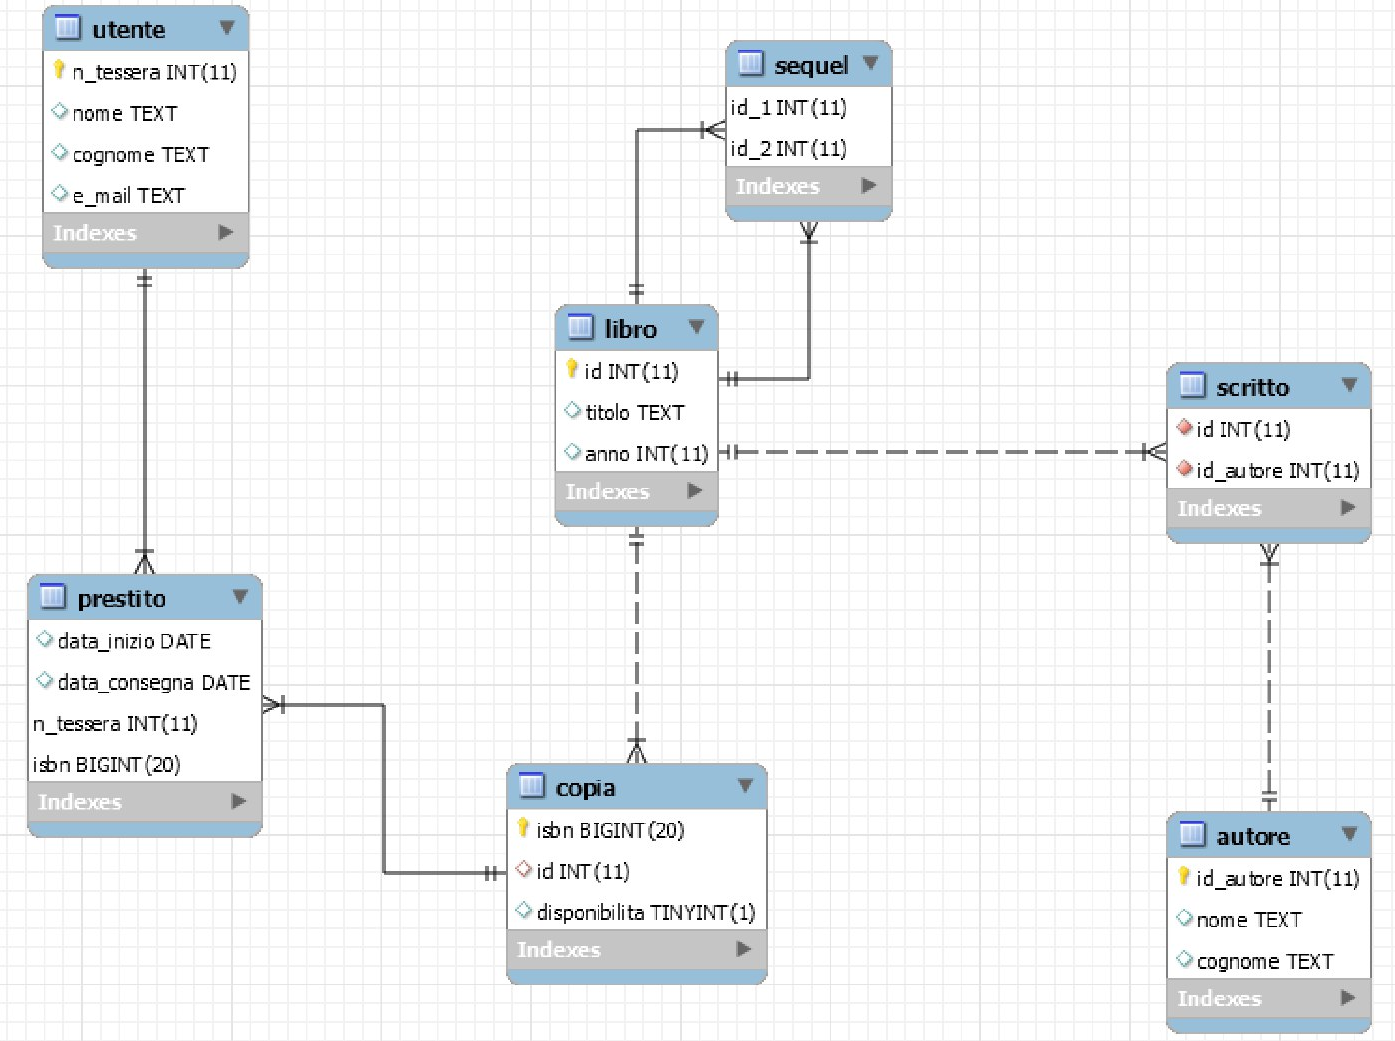
\includegraphics[width=0.7\linewidth]{images/ERdiagram}
	\caption[Schema ER]{Schema ER}
	\label{fig:re}
\end{figure}

Le entità utilizzate nel nostro progetto sono così descritte:

\begin{itemize}
	\item Utente, descrive la persona registrata e utilizzatrice del sito
	\item Libro, elemento che compone la nostra libreria online
	\item Copia, insieme di diverse edizioni di un libro
	\item Autore, colui che ha scritto il libro
\end{itemize}

Esse sono messe in relazione da:
\begin{itemize}
	\item Prestito, entità che relaziona utente con copia
	\item Sequel, entità che mette in relazione un libro con se stesso
	\item Scritto, entità che mette in relazione autore con libro
\end{itemize}

In particolare:
\begin{itemize}
	\item Un utente può richiedere in prestito una sola copia di un libro
	\item Un libro può essere presente in più copie o nessuna
	\item Una copia può trovarsi in due stati, disponibile o non
	\item Un libro può essere collegato ad un altro in quanto suo sequel
	\item Un libro può essere scritto da uno o più autori e un autore può scrivere uno o più libri
\end{itemize}

All’interno dell’applicazione è presente un package di controller che permette le operazioni di CRUD tra le classi sopra citate.

\section*{L'applicazione}
Per poter accedere all’applicazioni bisogna obbligatoriamente essere registrati, esistono due tipi di utente:

\begin{itemize}
	\item Amministratore
	\item Cliente
\end{itemize}

L’amministratore ha la facoltà di poter svolgere le operazioni di modifica e di delete all’interno del programma mentre il cliente può solo verificare la disponibilità di un libro ed eventualmente prenotarlo.

\end{document}
